%-------------------------------------------------------------------------------
\section{Introduction}\label{sec:introduction}
%-------------------------------------------------------------------------------
This document is intended to be a user documentation/manual of the sky
correction code SKYCORR developed within the framework of the Austrian
\acs{ESO} In-Kind SM project as described in the corresponding Statement of
Work document \cite{SM-SoW}.

The aim of the SKYCORR project is to provide an advanced instrument-independent
sky-correction tool that removes sky emission in science spectra by means of
sky spectra taken at a different time and sky location. The algorithm adapts a
reference sky spectrum to a science spectrum by correcting differences due to
temporal and spatial airglow variability and issues related with the instrument
or the data reduction\footnote{For multi-object and integral-field
spectroscopy, it could be prudent to correct with a reference sky spectrum
taken from the same exposure. In this case, SKYCORR would mainly be used to
correct for instrumental effects.}. The approach is based on a similar method
for SINFONI near-IR spectroscopic data described in Davies \cite{DAV07}.

This document is organised as follows: Section~\ref{sec:overview} gives a
brief overview on the project and the incorporated algorithms.
Section~\ref{sec:installation} provides information on the installation
procedure. Section~\ref{sec:running} contains a description of how to run the
code, the required input parameter file, and the output files.
Section~\ref{sec:method} explains the adapted sky correction method and the
airglow model in detail. Finally, the code performance is evaluated in
Section~\ref{sec:evaluation} by means of a test data set.

%-------------------------------------------------------------------------------
\section{Overview}\label{sec:overview}
%-------------------------------------------------------------------------------
%-------------------------------------------------------------------------------
\subsection{The Davies method}\label{sec:davies}
%-------------------------------------------------------------------------------
For spectroscopic instrument set-ups and observing programmes that do not
provide pure sky spectra in parallel to the desired object spectra (\eg\
two-dimensional long-slit spectra where the object does not cover the whole
slit), it is necessary to use sky spectra taken at a different time as the
science spectra for the sky correction. However, the strong variability of
airglow emission on time scales in the order of a few minutes can
cause unavoidable sky correction residua. Significant changes in the airglow
emission can also be expected for sky position differences in the order of a
few degrees or even less depending on the characteristics of possible wave
patterns. Moreover, different telescope positions and ambient conditions may
cause instrument flexures, which result in shifting of the sky with regard to
the science spectrum. Hence, the reference sky spectrum has to be adapted in
both, the flux and the wavelength regime, to allow a reasonable sky background
correction.

An illustration of this problem and a solution for SINFONI has been described
by Davies \cite{DAV07}. The airglow correction method proposed in this paper is
based on applying arbitrary sky spectra to science spectra by scaling
physically related OH line groups of the sky spectrum to the corresponding
groups in the science spectrum. Subsequently, the newly created scaled spectrum
is used for the sky correction. Specifically, the Davies method groups emission
lines from vibrational-rotational transitions resulting from non-thermal
excitation processes of the OH molecule and defines wavelength regions where
these groups dominate the airglow emission. These wavelength ranges are scaled
in the sky spectrum to match the corresponding flux in the object spectrum.
This approach only works for the line component of the sky emission. Since
object and sky continua cannot satisfyingly be separated, the sky continuum
cannot be adapted and has to be subtracted before the scaling procedure for the
line emission can start. Since the Davies method is restricted to OH airglow
lines beyond 1\,$\mu$m\footnote{The version 2.0 of Davies' code also allows
simple scaling of the strong O$_2$ band at 1.27\,$\mu$m. This feature is not
described in Davies \cite{DAV07}.}, it can only be applied in near-IR
wavelength regions where other line emission is negligible. This method has
been implemented for SINFONI (Modigliani et al. \cite{MOD07}).

%-------------------------------------------------------------------------------
\subsection{Improvements of the Davies method}
\label{sec:improvements}
%-------------------------------------------------------------------------------
In the framework of the SM subproject ``Advanced sky model'', an extended
semi-empirical model for airglow emission was developed (see \cite{SM01} User
Manual and Noll et al. \cite{NOL12}). It is based on the OH line list by
Rousselot et al. \cite{ROU00}. Also, it incorporates the empirical
--mainly optical-- line list by Hanuschik \cite{HAN03} and Cosby et al.
\cite{COS06} based on high-resolution UVES observations, and the HITRAN
database for molecular data \cite{HITRAN}. Additionally, five variability
classes were introduced for the entire line list (\ie\ green O\,I, Na\,D, red
O\,I, OH, and O$_2$, see Section~\ref{sec:airglow}) in order to take into
account intensity variations due to changes of the solar activity, the season,
and the time during the night. The variability correction recipes for the
different classes were calculated from 1189 VLT FORS sky spectra (Patat
\cite{PAT08}).

For SKYCORR, this model is extended by identifications of lines with similar
upper and lower electronic, vibrational, and/or rotational states that are
expected to vary in a very similar way (more similar than the lines belonging
to the relatively rough variability classes defined in Noll et al.
\cite{NOL12}). If the spectral resolution is given, the airglow emission
model with the improved line list (ranging from 0.3 to 2.5\,$\mu$m) allows
deriving the contributions of different line groups to the pixels of a sky
spectrum. Hence, in wavelength space overlapping groups can be handled by such
an implementation contrary to the Davies method, which uses fixed wavelength
intervals. The optimum scaling of the different line groups is then derived by
means of a fitting procedure that is not required for the simpler approach of
Davies. This fitting procedure also allows the wavelength grid to be adapted.
Similar to \cite{MOLECFIT}, the adaptation process is based on Chebyshev
polynomials and subpixel shifts instead of simple shifting by full pixels only.
In general, the new method should be applicable to all wavelength regions where
airglow emission plays an important role. Hence, apart from SINFONI, the
SKYCORR code is also appropriate for correcting spectroscopic observational
data from, \eg, ISAAC, X-Shooter, VIMOS, or FORS.

%-------------------------------------------------------------------------------
\subsection{Algorithm}\label{sec:algorithm}
%-------------------------------------------------------------------------------
The algorithm used by the SKYCORR code is sketched in
Figure~\ref{fig:skycorr_overview}. Its main purpose is the removal of sky
emission lines in a science spectrum by means of a scaled reference sky
spectrum. To this end, any continuum flux in the input science and reference
sky spectra has to be removed in advance. Hence, as a first step, pixels
belonging to lines and continuum have to be identified, separated, and masked
accordingly. The second step is a fit to continuum pixels only, which is
subtracted from the input spectrum to obtain a continuum-free spectrum. In the
third step, a weight mask for the different airglow line groups in the
reference sky spectrum is calculated incorporating the extended sky model
mentioned above. The actual line and wavelength fitting process is performed in
step four (incorporating the MPFIT library \cite{CMPFIT}). Here, the reference
sky line spectrum is fitted to the emission lines in the science spectrum.
Finally, the best-fit sky line spectrum and the uncorrected sky continuum
spectrum are subtracted from the input science spectrum. More details on this
approach can be found in Section~\ref{sec:method}.

%-------------------------------------------------------------------------------
\begin{figure}[ht]
  \begin{center}
    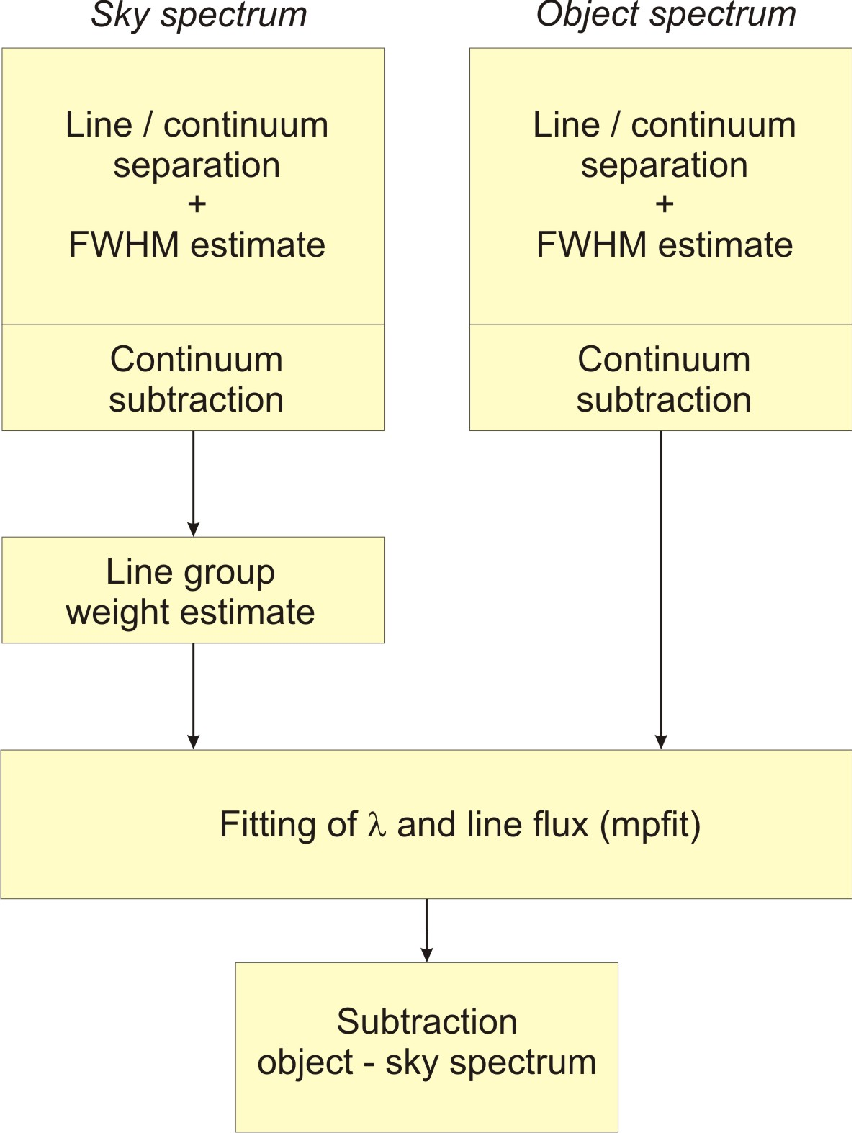
\includegraphics[width=0.9\textwidth]{figures/skycorr_workflow_scheme.png}
    \caption{{\it Overview of the SKYCORR project workflow}.}
    \label{fig:skycorr_overview}
  \end{center}
\end{figure}
%-------------------------------------------------------------------------------
